\documentclass{article}
% --- watermark (auto-inserted) ---
\usepackage{xcolor}
\usepackage{xfp}% \fpeval; in the kernel since 2022, harmless on older LaTeX
\usepackage{draftwatermark}
\newlength{\watermarkTextWidth}
\AddToHook{begindocument/end}{%
  \SetWatermarkText{\normalfont Generated by The Agentic Scientist}%
  \SetWatermarkFontSize{10pt}%
  \SetWatermarkLightness{0.85}%
  \settowidth{\watermarkTextWidth}{\normalfont\fontsize{10pt}{12pt}\selectfont Generated by The Agentic Scientist}%
  \edef\watermarkScale{\fpeval{0.8 * sqrt(\paperwidth**2 + \paperheight**2) / \watermarkTextWidth}}%
  \edef\watermarkAngle{\fpeval{atand(\paperheight/\paperwidth)}}%
  \SetWatermarkScale{\watermarkScale}%
  \SetWatermarkAngle{\watermarkAngle}%
}
% --- end watermark ---
 % For LaTeX2e
\usepackage{paper,times}

\usepackage{hyperref}
\usepackage{url}
\usepackage{amsmath,amssymb}
\usepackage{booktabs}
\usepackage{graphicx}
\usepackage{subcaption}

\title{Six Cheap Statistics versus Worst-Case Bounds:\\Predicting Random-Walk Cover Times on Small Graphs}
\iclrfinalcopy
\author{The Agentic Scientist}

\newcommand{\Ccov}{C}
\newcommand{\diam}{\mathrm{diam}}

\begin{document}
\maketitle

\begin{abstract}
The classical cover-time bounds $2m(n-1)$ and $(4/27)n^3$ hold for every graph but can be loose on concrete small graphs. We ask whether six cheap statistics, namely vertex and edge counts, mean, maximum and minimum degree, and diameter, predict the expected cover time of connected graphs with $5\le n\le 30$ more accurately, and how the error depends on graph type. An untuned log-linear ridge regression is fitted to Monte Carlo labels on 117 graphs from ten synthetic families. It is scored on 116 held-out graphs that are isomorphism-disjoint from the training graphs, with a paired two-level bootstrap. Its mean absolute log error is 0.183 (95\% CI 0.167--0.207), a typical error factor of 1.20, against 1.397 (factor 4.0) for the better bound. The paired advantage is significant in 9 of 10 families and largest where the bounds are loosest (complete, Erd\H{o}s--R\'enyi, random 3-regular). On lollipops, where the cubic bound is nearly tight, the advantage is not statistically clear. Fitted prediction helps most far from the worst case, but it carries no guarantee outside the studied families and sizes.
\end{abstract}

% ===================================================================
\section{Introduction}
\label{sec:intro}

Start a simple random walk at a vertex of a connected undirected graph $G=(V,E)$ and let it step to a uniformly random neighbour until every vertex has been visited. The expected number of steps is the \emph{cover time}. It governs randomized graph exploration and the space-efficient connectivity algorithm of \citet{Aleliunas1979RandomWU}, and more generally any procedure that must touch every state of a reversible Markov chain \citep{Lovász2001RandomWO}. The theory is mature. \citet{Aleliunas1979RandomWU} showed that the cover time of any connected graph with $n$ vertices and $m$ edges is at most $2m(n-1)$. Feige later showed that the worst case over all $n$-vertex graphs is $(4/27)n^3$ to leading order, attained asymptotically by lollipop graphs (for these worst-case results see the survey of \citealp{Lovász2001RandomWO}), and that every connected graph needs at least about $n\ln n$ steps \citep{Feige1995ATL}. These results are tight \emph{over the class of all graphs}. For a specific small graph that is far from the extremal shape, both bounds can overshoot the true cover time by a large factor.

Practitioners who need a number for a given small graph, for example to set a walk budget or sanity-check a simulator, therefore face a gap. The worst-case bounds are cheap but loose. Exact computation or long simulation is accurate but needs the whole graph and substantial compute. Tighter graph-aware bounds also need full structural information, such as all pairwise hitting times or effective resistances \citep{Chandra1989TheER}. This motivates a narrow empirical question that the literature leaves open:

\emph{For connected graphs with at most 30 vertices, can a handful of easily computed statistics (vertex count, edge count, mean, maximum and minimum degree, and diameter) predict the cover time more accurately than the generic bounds? On which kinds of graph is such a predictor reliable, and where does it fail?}

We answer with a controlled, reproducible measurement rather than a new model. The predictor is a deliberately simple, untuned log-linear ridge regression on the logarithms of the six statistics plus one interaction term. It is fitted on Monte Carlo estimates of the uniform-start cover time. All accuracy claims come from a single sealed evaluation on held-out graphs that are isomorphism-disjoint from the training graphs, drawn from ten synthetic families: paths, cycles, stars, complete graphs, 2D grids, binary trees, lollipops, random trees, Erd\H{o}s--R\'enyi graphs and random 3-regular graphs. Uncertainty is quantified by a two-level bootstrap that resamples both graphs and Monte Carlo walks. Comparisons with each bound use paired resamples.

\paragraph{Contributions.}
\begin{itemize}
\item \textbf{A calibrated accuracy comparison with the generic bounds.} On held-out graphs, the six-statistic predictor has family-weighted mean absolute log error 0.183 (95\% CI 0.167--0.207). The best of $2m(n-1)$ and $(4/27)n^3$ has error 1.397, and the paired difference has CI $[-1.303,-1.130]$ (\S\ref{sec:main}). A size-only fitted reference, a constant predictor and a permuted-feature control show that the gain depends on the degree and diameter statistics and on each graph's own feature vector (\S\ref{sec:controls}).
\item \textbf{A family-resolved reliability map.} We report per-family errors and paired gains with confidence intervals. The predictor is most accurate on stars, random 3-regular graphs, random trees and paths, and least accurate on complete, grid and Erd\H{o}s--R\'enyi graphs. Its advantage over the bounds is significant in nine families and not statistically clear on lollipops (\S\ref{sec:family}).
\item \textbf{A mechanistic reading of where fitted prediction helps.} The per-family gain tracks the slack of the best bound. Gains are smallest on the two families near the bounds' extremal shapes (lollipop and path). They are largest on complete graphs, which attain the $n\ln n$ lower-bound regime, and on Erd\H{o}s--R\'enyi and random 3-regular graphs, where the measured bound slack is similarly large (\S\ref{sec:discussion}).
\end{itemize}

% ===================================================================
\section{Background and Related Work}
\label{sec:related}

\paragraph{Cover time and its generic bounds.}
For a connected graph $G$ with $n$ vertices and $m$ edges, let $\tau_{\mathrm{cov}}$ be the first time a simple random walk has visited every vertex. Following the evaluation protocol in \S\ref{sec:protocol}, we study the \emph{uniform-start} cover time
\begin{equation}
\Ccov(G) \;=\; \frac{1}{n}\sum_{v\in V}\mathbb{E}_v\!\left[\tau_{\mathrm{cov}}\right],
\end{equation}
which averages over a uniformly random starting vertex. The spanning-tree argument of \citet{Aleliunas1979RandomWU} gives $\Ccov(G)\le 2m(n-1)$ for every start vertex. The bound overestimates dense graphs badly: for the complete graph $K_n$ it is $n(n-1)^2$, whereas $\Ccov(K_n)=(n-1)H_{n-1}$, where $H_k$ is the $k$-th harmonic number \citep{Lovász2001RandomWO}. Feige's upper bound $\tfrac{4}{27}n^3+o(n^3)$ is the exact worst case over $n$-vertex graphs and is approached by lollipops, i.e.\ a clique of about $2n/3$ vertices joined to a path; the survey of \citet{Lovász2001RandomWO} places this result alongside the extremal hitting-time analysis of the lollipop. At the other extreme, every connected graph has cover time at least $(1-o(1))\,n\ln n$, which the complete graph approaches \citep{Feige1995ATL}. The ratio between the two extremes grows like $n^2/\ln n$. Even at $n\le 30$, true cover times therefore span orders of magnitude across graph shapes. A bound that depends only on $n$ and $m$ cannot be accurate across that whole range.

\paragraph{Graph-aware characterizations.}
Tighter estimates use more structure. Matthews' method, presented in the survey of \citet{Lovász2001RandomWO}, bounds the cover time by the maximum hitting time times $H_{n-1}$. \citet{Chandra1989TheER} showed that commute times equal $2m$ times the effective resistance between the endpoints. As a result, the cover time lies within a logarithmic factor of $m\,R_{\max}$, where $R_{\max}$ is the largest effective resistance between any two vertices. Since $R_{\max}$ is at most the diameter, the product $m\cdot\diam(G)$ is a natural cheap proxy for this resistance scale. Exact hitting times and effective resistances need a linear solve on the full adjacency matrix, so they are not ``cheap statistics'' in our sense. We still include a Matthews-type reference (maximum hitting time times $H_{n-1}$) as a graph-aware comparison point. The survey of \citet{Lovász2001RandomWO} collects the classical closed forms for paths, cycles, complete graphs and stars. These closed forms are used here only to check the simulator (\S\ref{sec:protocol}).

\paragraph{Positioning.}
Prior work on cover time, as collected in the survey of \citet{Lovász2001RandomWO}, is overwhelmingly analytic: it derives bounds that hold for all graphs, and closed forms or growth rates for particular families such as paths, cycles, stars and complete graphs. We do not rely on finer asymptotic results for random families; for random 3-regular, Erd\H{o}s--R\'enyi and grid graphs, all statements in this paper about regimes rest on our own measurements. We are not aware of a controlled, held-out measurement of how well a few global statistics predict the cover time of concrete small graphs, broken down by graph family, with Monte Carlo and graph-sampling uncertainty propagated into the comparison. Our study is complementary to the analytic results, not a substitute. Bounds come with guarantees, whereas a fitted predictor is only as good as the match between training and test distributions. We therefore treat the bounds \emph{as predictors}, i.e.\ we score them by how close they are to the true value, and we limit every claim to the evaluated families and sizes.

% ===================================================================
\section{Method}
\label{sec:method}

\begin{figure}[t]
\centering

\includegraphics[width=0.95\textwidth,height=0.3\textheight,keepaspectratio]{figures/overview_concept.png}
\caption{Overview of the study. Graphs from ten synthetic families ($5\le n\le 30$) are reduced to six cheap statistics. A log-linear ridge regression fitted on Monte Carlo cover-time labels maps them to a predicted cover time, which is compared with the generic bounds $2m(n-1)$ and $(4/27)n^3$. Every predictor is scored on held-out graphs that are isomorphism-disjoint from the training graphs, using a paired two-level bootstrap over graphs and walks.}
\label{fig:overview}
\end{figure}

\subsection{Problem setup}
\label{sec:setup}
The input to a predictor is a training set of connected graphs, each described by the feature vector
\begin{equation}
x(G) = \bigl(n,\; m,\; \bar d = 2m/n,\; d_{\max},\; d_{\min},\; \diam(G)\bigr)
\end{equation}
and a Monte Carlo estimate $\hat \Ccov(G)$ of its uniform-start cover time with standard error. After fitting, the predictor sees only $x(G)$ for each held-out graph. It sees no adjacency information, family label, graph identifier or held-out label, and it must return a strictly positive prediction $\hat y(G)$. The error on one graph is the absolute log ratio, capped at $\ln 1000$:
\begin{equation}
e(G) = \min\bigl(\,|\ln \hat y(G) - \ln \hat \Ccov(G)|,\; \ln 1000\bigr).
\end{equation}
Errors are averaged within each family, and the ten family means are averaged with equal weight. We call this family-weighted average the \emph{mean absolute log error}; lower is better. Equal family weighting stops the large random families from dominating the score. A mean absolute log error of $\epsilon$ means a typical multiplicative error of $e^{\epsilon}$; we use the term geometric-mean error factor for $e^{\epsilon}$ in this informal sense. The log scale is natural because cover times across families differ by orders of magnitude, and because over- and underestimating by the same factor should cost the same.

\subsection{Design rationale}
\label{sec:rationale}
The classical results suggest that, within a fixed structural regime, the cover time behaves roughly like a product of powers of size and geometry. Examples are $(n-1)H_{n-1}\approx n\ln n$ for complete graphs, $n(n-1)/2$ for cycles, $\Theta(n^2)$ for paths, $\Theta(n^3)$ for lollipops, and $m\,R_{\max}$ up to a logarithmic factor in general \citep{Feige1995ATL,Chandra1989TheER,Lovász2001RandomWO}. A product of powers is linear in log space. This motivates a log-linear model in $\ln n$, $\ln m$ and $\ln \diam$. Degree statistics are added because they separate regimes with the same $(n,m)$. For example, a star and a path with the same $n$ have equal $m$ but very different $d_{\max}$ and diameter, and their cover times differ by a factor that grows roughly like $n/\ln n$. The minimum degree reflects bottlenecks such as pendant paths, which dominate lollipop cover times. An interaction term $\ln n\cdot\ln\diam$ lets the effective exponent on the diameter vary with size. This allows, for instance, a different diameter dependence for long thin graphs than for compact ones. We expected this representation to capture most of the variation \emph{between} regimes, which is exactly what $n$- and $m$-only bounds miss. We also expected it to fit less well within families whose cover time is not a single power law in these statistics. These are design expectations; we do not isolate the contribution of individual terms (\S\ref{sec:limits}).

\subsection{The statistics-only predictor}
\label{sec:predictor}
The predictor regresses $\ln \hat \Ccov$ on the design vector
\begin{equation}
z(G) = \bigl(\ln n,\ \ln m,\ \ln \bar d,\ \ln d_{\max},\ \ln d_{\min},\ \ln \diam,\ \ln n\cdot\ln \diam\bigr).
\end{equation}
Each column is standardized with the training mean and standard deviation; a standard deviation below $10^{-12}$ is replaced by 1. An unpenalized intercept is added. The coefficients solve the ridge system $(Z^\top Z+\lambda D)\beta = Z^\top \ln \hat{\mathbf C}$ with $\lambda=10^{-3}$, where $D$ is the identity with a zero in the intercept position. At test time the predictor returns $\hat y = \exp\bigl(\mathrm{clip}(\beta^\top \tilde z, -50, 50)\bigr)$, where $\tilde z$ is the standardized design vector with a leading 1. Non-finite values fall back to the mean training log label. The source is at \texttt{source\_evidence/downstream/program/src/program.py}, lines 45--83. The small ridge term mainly resolves an exact collinearity: $\ln\bar d = \ln 2 + \ln m - \ln n$, so the design matrix is rank-deficient without it. The predictor ignores the Monte Carlo standard errors and uses no hyperparameter search, cross-validation or family information. Its predictions are a deterministic, pure function of the six statistics of each row.

\subsection{Compared predictors}
\label{sec:compared}
All comparison predictors are computed by the evaluator on the same held-out graphs (\texttt{task/evaluate\_final.py}, \texttt{baseline\_predictions}).
\begin{itemize}
\item \textbf{Generic bounds used as predictors:} $2m(n-1)$ \citep{Aleliunas1979RandomWU}; the leading term $(4/27)n^3$ of Feige's upper bound (see \citealp{Lovász2001RandomWO}); and their pointwise minimum, called the \emph{best bound}. The best bound is the strongest predictor that uses only the generic bounds and is our primary comparator.
\item \textbf{Matthews-type reference} (Matthews' bound; see \citealp{Lovász2001RandomWO}): the exact maximum hitting time (from a linear solve on the full transition matrix) times $H_{n-1}$. It needs the whole graph, so it marks what full structural information gives a bound-based predictor.
\item \textbf{Size-only fitted reference:} ordinary least squares of $\ln\hat\Ccov$ on $(1,\ln n,\ln m)$ over the same training labels. It shows how much is explained by size alone, without degree or diameter. It is an evaluator-defined reference, not a training-matched ablation of our predictor.
\item \textbf{Constant predictor:} the geometric mean of the training labels. It is the feature-free baseline.
\item \textbf{Permuted-feature control:} our fitted predictor applied to a derangement of the held-out feature rows, so that each graph is scored with another graph's statistics. It tests whether accuracy comes from each graph's own statistics rather than from matching the overall label distribution.
\end{itemize}

\subsection{Evaluation protocol}
\label{sec:protocol}

\begin{table}[t]
\centering
\caption{Graph families and pool sizes. Deterministic families are split by $n \bmod 3$ (grids by shape index $\bmod 3$). The residue class not shown is reserved for a separate development pool. Random families are drawn from independent seeds and resampled until non-isomorphic to every catalogue graph and to the other pools. Counts are derived from the evaluator's catalogue and plane configuration.}
\label{tab:roster}
\small
\begin{tabular}{llrr}
\toprule
Family & Construction ($5\le n\le 30$) & Train & Held-out \\
\midrule
Path, cycle, star, complete, binary tree & one graph per $n$ & 9 each & 9 each \\
2D grid & $a\times b$, $2\le a\le 5$, $a\le b\le 3a$ & 6 & 5 \\
Lollipop & clique $K_k$ + path, $k\in\{\lceil n/2\rceil,\lceil 2n/3\rceil\}$ & 18 & 18 \\
Random tree & uniform labelled tree (Pr\"ufer) & 16 & 16 \\
Erd\H{o}s--R\'enyi & $p\sim U[2\ln n/n,\ \max(0.5, 2\ln n/n)]$, connected & 16 & 16 \\
Random 3-regular & configuration model, simple, connected & 16 & 16 \\
\midrule
Total & & 117 & 116 \\
\bottomrule
\end{tabular}
% @evidence[[analysis/roster.json#train.total]] @evidence[[analysis/roster.json#final_eval.total]]
\end{table}

\paragraph{Graph pools.} Table~\ref{tab:roster} lists the ten families. Graphs in the seven deterministic families are assigned to pools by a fixed rule on $n$ (or on the shape index for grids), so no shape appears in both training and held-out pools. The three random families are generated from independent seeds; any draw isomorphic to a catalogue graph or to a graph in another pool is rejected and redrawn. The evaluator verified zero isomorphic overlap between the held-out pool and both the training and development pools. % @evidence[[paper_data.json#final_evaluation.metrics.iso_overlap_count]]

\paragraph{Monte Carlo labels.} Each graph is labelled by simulating 256 independent walks, each from a uniformly random start vertex. The label $\hat\Ccov$ is the mean cover time and its standard error is the sample standard deviation divided by $\sqrt{256}$. % @evidence[[analysis/roster.json#walks_per_graph]]
Walks are capped at $40\cdot 2m(n-1)$ steps; no training or held-out walk reached the cap. The median relative standard error of the held-out labels is 0.033. % @evidence[[paper_data.json#final_evaluation.metrics.capped_walks]] @evidence[[paper_data.json#final_evaluation.metrics.mc_rel_se_median]]
Before labelling, the simulator is checked against three closed forms: $\Ccov(C_{12}) = 66$, $\Ccov(K_{10}) = 9H_9$, and the uniform-start cover time of $P_{10}$. Each estimate must agree within four standard errors.

\paragraph{Episodes and controls.} An evaluation episode resets the predictor with a seed, fits it on the 117 training graphs, and issues three prediction requests on the 116 held-out graphs in an evaluator-private random order. The requests are the main query, the permuted-feature control, and a reordered copy of the main query. The reordered copy tests that predictions are a pure function of each row. The maximum relative difference between the main and reordered predictions was 0. % @evidence[[paper_data.json#final_evaluation.metrics.order_invariance_max_rel_diff]]
Three episodes were run with reset seeds 211, 212 and 213, and none failed. Because the predictor is deterministic and the labels are fixed, all three episodes gave identical errors: the seed range of the main error is 0. % @evidence[[paper_data.json#final_evaluation.evidence.episodes]] @evidence[[paper_data.json#final_evaluation.metrics.final_main_log_err_seed_range]]
This shows reproducibility; it is \emph{not} evidence of robustness to new graph or label draws.

\paragraph{Uncertainty.} Confidence intervals come from a two-level bootstrap with 1000 replicates. Within each family, held-out graphs are resampled with replacement, and each resampled graph's 256 walk times are resampled to form a bootstrap label. Errors are then recomputed for every predictor on the same replicate, and 95\% percentile intervals are reported. For comparisons, the paired difference (our predictor's error minus the comparator's) is computed on each replicate. The interval therefore reflects both graph-sampling and Monte Carlo variability, and shared variability cancels in the paired comparison. A paired interval that excludes zero is what we call a significant difference.

% ===================================================================
\section{Results}
\label{sec:results}

\subsection{Main result: accuracy relative to the generic bounds}
\label{sec:main}

\begin{table}[t]
\centering
\caption{Held-out accuracy of all predictors (family-weighted mean absolute log error, lower is better; the error factor is $e^{\text{error}}$). Paired $\Delta$ is our predictor's error minus the comparator's, with 95\% two-level bootstrap CI; dashes mark comparisons for which the evaluator reports no paired interval. ``Full graph'' marks predictors that need the adjacency matrix.}
\label{tab:main}
\small
\begin{tabular}{lcccc}
\toprule
Predictor & Inputs & Error & Factor & Paired $\Delta$ (95\% CI) \\
\midrule
\textbf{Six-statistic log-linear ridge} & 6 statistics & \textbf{0.183} [0.167, 0.207] & 1.20 & --- \\
Size-only OLS $(\ln n,\ln m)$ & $n, m$ & 0.526 & 1.69 & $[-0.391,\,-0.288]$ \\
Constant (training geo.\ mean) & none & 0.942 & 2.56 & --- \\
Permuted-feature control & other graph's stats & 1.261 & 3.53 & $[-1.196,\,-0.955]$ \\
\midrule
Matthews ref.\ ($\max H\cdot H_{n-1}$) & full graph & 0.605 & 1.83 & --- \\
Best bound $\min\{2m(n-1), \tfrac{4}{27}n^3\}$ & $n, m$ & 1.397 & 4.04 & $[-1.303,\,-1.130]$ \\
$(4/27)n^3$ & $n$ & 1.604 & 4.97 & --- \\
$2m(n-1)$ & $n, m$ & 1.836 & 6.27 & --- \\
\bottomrule
\end{tabular}
% @evidence[[paper_data.json#final_evaluation.metrics.final_main_log_err]] @evidence[[paper_data.json#final_evaluation.metrics.final_main_log_err_ci_low]] @evidence[[paper_data.json#final_evaluation.metrics.final_main_log_err_ci_high]]
% @evidence[[paper_data.json#final_evaluation.metrics.ols_ref_log_err]] @evidence[[paper_data.json#final_evaluation.metrics.constant_log_err]] @evidence[[paper_data.json#final_evaluation.metrics.permuted_feature_log_err]]
% @evidence[[paper_data.json#final_evaluation.metrics.matthews_ref_log_err]] @evidence[[paper_data.json#final_evaluation.metrics.best_bound_log_err]] @evidence[[paper_data.json#final_evaluation.metrics.feige_lead_log_err]] @evidence[[paper_data.json#final_evaluation.metrics.aklrr_log_err]]
% @evidence[[paper_data.json#final_evaluation.metrics.delta_vs_best_bound_ci_low]] @evidence[[paper_data.json#final_evaluation.metrics.delta_vs_ols_ref_ci_low]] @evidence[[paper_data.json#final_evaluation.metrics.delta_permuted_minus_main_ci_low]]
\end{table}

\begin{figure}[t]
\centering
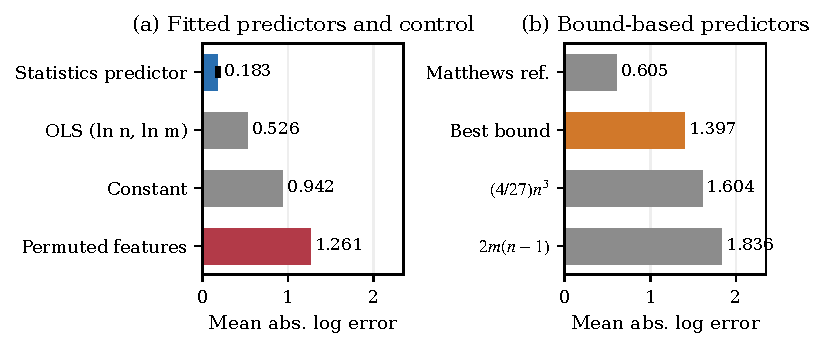
\includegraphics[width=0.95\textwidth]{figures/plane_level_comparison.pdf}
\caption{Held-out mean absolute log error by predictor. (a) Fitted predictors and the permuted-feature control; the error bar on our predictor is its 95\% two-level bootstrap CI. (b) Bound-based predictors. The Matthews reference needs the full graph. The x-axis is shared across panels.}
\label{fig:plane}
\end{figure}

Table~\ref{tab:main} and Figure~\ref{fig:plane} summarize held-out accuracy. The six-statistic predictor has mean absolute log error 0.183 (95\% CI 0.167--0.207), so a typical prediction is off by a factor of about 1.20 (CI about 1.18--1.23). The best of the two generic bounds has error 1.397, a typical factor of about 4.0. % @evidence[[analysis/derived_metrics.json#geo_ratio_predictor]] @evidence[[analysis/derived_metrics.json#geo_ratio_best_bound]]
The paired difference is $-1.215$ log units, with 95\% CI $[-1.303,-1.130]$. % @evidence[[analysis/derived_metrics.json#best_bound_minus_predictor_plane]] @evidence[[paper_data.json#final_evaluation.metrics.delta_vs_best_bound_ci_high]]
It is far from zero: on the log scale, the predictor removes about 87\% of the best bound's error. % @evidence[[analysis/derived_metrics.json#fraction_of_best_bound_error_removed]]
 Each bound on its own does worse than their minimum ($(4/27)n^3$: 1.604; $2m(n-1)$: 1.836), because each is loose on a different part of the graph space (\S\ref{sec:discussion}).

The answer to the first research question is therefore yes, within the evaluated regime. Six statistics, combined by a model fitted on in-distribution labels, predict small-graph cover times far more accurately than the generic bounds evaluated at the same graphs. This should not be misread. The bounds hold for every connected graph, and the comparison scores them only on closeness to the true cover time, which they were never designed to optimize. The predictor offers no guarantee in either direction. Its errors are two-sided, and it can underestimate.

A more demanding comparison is the Matthews-type reference, which uses exact hitting times from the full transition matrix. Its error is 0.605, lower than either generic bound. The six-statistic predictor has a lower point-estimate error (0.183 vs.\ 0.605), but the evaluator reports no paired interval for this comparison, so we do not attach a significance statement to it. One possible explanation, which we have not tested, is that a fitted model is not constrained to overestimate: it can learn the typical ratio between cover time and its scale, whereas a bound must cover that ratio with a worst-case constant.

\subsection{Which inputs carry the signal: fitted references and controls}
\label{sec:controls}
Three references bracket what the statistics contribute. A constant prediction (the training geometric mean) has error 0.942, which is already lower than both generic bounds. This underlines how far the bounds are from typical small-graph cover times. Fitting a size-only power law in $n$ and $m$ lowers the error to 0.526. Adding the degree and diameter statistics, in our predictor, lowers it further to 0.183. The paired interval for the difference between our predictor and the size-only reference is $[-0.391,-0.288]$. % @evidence[[paper_data.json#final_evaluation.metrics.delta_vs_ols_ref_ci_high]]
The size-only reference differs from our predictor in its feature set (and in a negligible ridge term), so the comparison indicates that degree and diameter carry substantial information beyond size. Because it is not a one-feature-at-a-time ablation, it does not show which of these statistics matters most.

The permuted-feature control applies the same fitted predictor to statistics taken from a different held-out graph. Its error rises to 1.261, worse than the constant predictor. The paired increase relative to the correctly matched predictions has 95\% CI $[0.955, 1.196]$. % @evidence[[paper_data.json#final_evaluation.metrics.delta_permuted_minus_main_ci_high]]
Accuracy therefore depends on each graph's own statistics, not merely on reproducing the marginal distribution of labels. The pure-function check gave zero discrepancy, so predictions are not affected by request order or batch composition.

How much of the remaining error could be label noise? The median relative standard error of the Monte Carlo labels is 0.033. A relative error of this size is about 0.033 in log units, a small fraction of the 0.183 error. The predictor's residual error is therefore dominated by misfit of the log-linear surface, not by noise in the labels. The bootstrap intervals include the label noise.

\subsection{Per-family reliability}
\label{sec:family}

\begin{figure}[t]
\centering
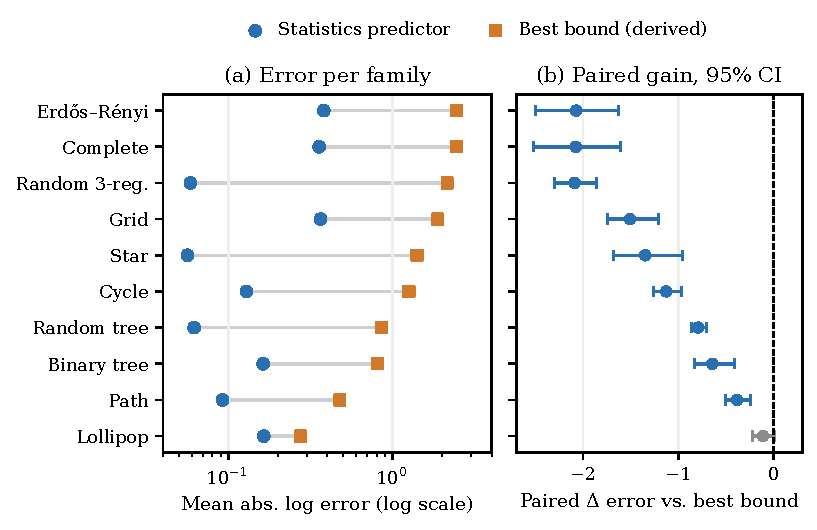
\includegraphics[width=\textwidth]{figures/per_family_reliability.pdf}
\caption{Per-family reliability map on held-out graphs; families are sorted by the best bound's error (bound slack), increasing upward. (a) Mean absolute log error of our predictor (circles) and of the best bound (squares, log scale). The best-bound error per family is derived as our predictor's error minus the paired difference. (b) Paired difference in error (our predictor minus best bound) with 95\% two-level bootstrap CI. Blue intervals exclude zero; the grey lollipop interval includes zero.}
\label{fig:family}
\end{figure}

Figure~\ref{fig:family} and Table~\ref{tab:family} in the Supplementary Information address the second research question. The predictor's own error varies by a factor of almost seven across families. % @evidence[[analysis/derived_metrics.json#per_family_error_spread_ratio]]
 It is lowest on stars (0.056), random 3-regular graphs (0.059), random trees (0.062) and paths (0.092), all within about 10\% of the true value in typical ratio terms. % @evidence[[paper_data.json#final_evaluation.metrics.final_log_err_star]] @evidence[[paper_data.json#final_evaluation.metrics.final_log_err_random_regular3]] @evidence[[paper_data.json#final_evaluation.metrics.final_log_err_random_tree]] @evidence[[paper_data.json#final_evaluation.metrics.final_log_err_path]]
Cycles (0.129), binary trees (0.163) and lollipops (0.164) are intermediate. % @evidence[[paper_data.json#final_evaluation.metrics.final_log_err_cycle]] @evidence[[paper_data.json#final_evaluation.metrics.final_log_err_binary_tree]] @evidence[[paper_data.json#final_evaluation.metrics.final_log_err_lollipop]]
The predictor is least reliable on complete graphs (0.357), 2D grids (0.364) and Erd\H{o}s--R\'enyi graphs (0.381), where typical errors are 40--46\% in ratio terms. % @evidence[[paper_data.json#final_evaluation.metrics.final_log_err_complete]] @evidence[[paper_data.json#final_evaluation.metrics.final_log_err_grid]] @evidence[[paper_data.json#final_evaluation.metrics.final_log_err_erdos_renyi]]
These three families contribute about 60\% of the family-weighted total. % @evidence[[analysis/derived_metrics.json#share_of_total_complete_grid_er]]
The evaluator reports no confidence intervals for the per-family errors themselves, so we make no claims about the ordering among families with similar errors.

The paired gain over the best bound (Figure~\ref{fig:family}b) has a 95\% interval excluding zero in 9 of 10 families. % @evidence[[analysis/derived_metrics.json#n_families_ci_excludes_zero]]
It is largest on random 3-regular graphs ($-2.088$, CI $[-2.303,-1.859]$), complete graphs ($-2.076$, CI $[-2.520,-1.608]$) and Erd\H{o}s--R\'enyi graphs ($-2.072$, CI $[-2.494,-1.626]$). % @evidence[[paper_data.json#final_evaluation.metrics.delta_vs_best_bound_random_regular3]] @evidence[[paper_data.json#final_evaluation.metrics.delta_vs_best_bound_complete]] @evidence[[paper_data.json#final_evaluation.metrics.delta_vs_best_bound_erdos_renyi]]
On these families the best bound is off by a typical factor of 8--12. Grids ($-1.507$), stars ($-1.347$) and cycles ($-1.126$) follow. % @evidence[[paper_data.json#final_evaluation.metrics.delta_vs_best_bound_grid]] @evidence[[paper_data.json#final_evaluation.metrics.delta_vs_best_bound_star]] @evidence[[paper_data.json#final_evaluation.metrics.delta_vs_best_bound_cycle]]
The gains on random trees ($-0.793$), binary trees ($-0.643$) and paths ($-0.384$, CI $[-0.502,-0.238]$) are smaller but clearly nonzero. % @evidence[[paper_data.json#final_evaluation.metrics.delta_vs_best_bound_random_tree]] @evidence[[paper_data.json#final_evaluation.metrics.delta_vs_best_bound_binary_tree]] @evidence[[paper_data.json#final_evaluation.metrics.delta_vs_best_bound_path]]
On lollipops the point estimate still favours the predictor ($-0.111$), but the interval $[-0.225, 0.013]$ includes zero, so the evaluation shows \emph{no statistically clear advantage} on this family. % @evidence[[paper_data.json#final_evaluation.metrics.delta_vs_best_bound_lollipop]] @evidence[[paper_data.json#final_evaluation.metrics.delta_vs_best_bound_lollipop_ci_low]] @evidence[[paper_data.json#final_evaluation.metrics.delta_vs_best_bound_lollipop_ci_high]]
This is not evidence that the predictor is worse than the bound on lollipops. It means only that the measurement cannot separate the two.

The two views do not align. The families on which the predictor is least accurate (complete, Erd\H{o}s--R\'enyi, grid) are also among those on which it gains the most over the bound. Low predictor error and high gain over the bound are distinct properties. Reliability, i.e.\ how close the prediction is to the truth, is a property of the fit. Advantage depends mostly on how loose the bound is.

% ===================================================================
\section{Discussion: Where Cheap Statistics Suffice}
\label{sec:discussion}

\paragraph{Gains track bound slack.}
Sorting families by the best bound's error (Figure~\ref{fig:family}a) gives an almost monotone pattern in the gains. The derived best-bound error is smallest on lollipops (0.275) and paths (0.476), the two families whose shapes are closest to the extremal constructions for the cubic and spanning-tree bounds. It is largest on complete (2.433) and Erd\H{o}s--R\'enyi graphs (2.453). % @evidence[[analysis/derived_metrics.json#per_family]]
A lollipop with a clique of about $2n/3$ vertices is the shape that asymptotically attains $(4/27)n^3$ \citep{Lovász2001RandomWO}. When a bound is nearly tight for a family, no predictor can beat it by much on that family. When a family lives near the opposite extreme, the bound must overshoot by a factor that grows with $n$, and any reasonable fitted model gains a lot. The latter case is exemplified by complete graphs, whose cover time $(n-1)H_{n-1}$ sits at the $n\ln n$ lower-bound regime \citep{Lovász2001RandomWO,Feige1995ATL}. Erd\H{o}s--R\'enyi and random 3-regular graphs show a similarly large bound slack in our measurements (Table~\ref{tab:family}); we read this as consistent with a near-$n\ln n$ regime for these families at $n\le 30$, but we did not test that reading separately. Our predictor does not need to understand the extremal combinatorics. It only needs to place a graph on the right scale, and the six statistics are enough for that.

\paragraph{Why the predictor is accurate on some families and not others (hypotheses).}
The following explanations are consistent with the measurements but were not tested by ablation. \emph{Low error} on stars, paths, cycles and random 3-regular graphs may reflect families whose cover time is close to a single power law in $(n,m,\diam,d_{\max})$ and whose members have distinctive statistic vectors. For example, stars are identified by $d_{\max}=n-1$ and $\diam=2$, and paths by $\diam=n-1$. \emph{Higher error} on complete graphs may arise because all complete graphs have $\diam=1$, which makes the interaction term vanish. The model must then express the $n\ln n$ growth through $\ln n$ and $\ln m$ alone, sharing coefficients with sparse families of very different growth. For Erd\H{o}s--R\'enyi graphs, the sampled edge density ranges from just above the connectivity threshold to $p=0.5$, so cover times move between sparse-tree-like and dense regimes, and the minimum degree only partly captures local bottlenecks. Grids contribute only six training graphs, with shapes from square to elongated. Their cover time may not follow a single power law in these statistics at this scale, which a log-linear surface cannot reproduce. Each of these hypotheses predicts that adding family-appropriate scaling terms (e.g.\ $n H_n$, $m\cdot\diam/d_{\min}$) would reduce the corresponding family error. That experiment is not part of the evidence reported here.

\paragraph{An intrinsic ceiling for statistics-only predictors.}
Twelve held-out graphs share their exact six-statistic vector with at least one other graph in the training or held-out pool. % @evidence[[paper_data.json#final_evaluation.metrics.feature_collision_count]]
Any predictor that sees only these statistics must give such graphs identical predictions, even when their cover times differ. Non-isomorphic graphs with equal $(n,m,\bar d, d_{\max}, d_{\min},\diam)$ can arise, for example, among trees with equal size, maximum degree and diameter. The evaluator does not report which families the collisions fall in, so we do not attribute them. This sets a floor, of unknown size, on the error of any statistics-only method on this distribution. It also suggests that richer but still cheap statistics, such as degree variance or the number of leaves, could help.

\paragraph{Practical reading.}
For a practitioner with a small graph from one of the evaluated families, the six-statistic predictor gives a point estimate typically within about 20\% of the expected cover time. It is more reliable on tree-like, regular and star-like graphs than on dense, random or grid graphs. When a guaranteed budget is required, the generic bounds remain the right tool, and their slack can be read off Figure~\ref{fig:family}a: for lollipop-like graphs the cheaper of the two bounds is already accurate to within a typical factor of about 1.3.

% ===================================================================
\section{Limitations}
\label{sec:limits}

\paragraph{Scope.} All graphs are synthetic, connected, and have $5\le n\le 30$ vertices from ten named families. The target is the uniform-start expected cover time; worst-start cover time, cover-and-return time and partial cover were not studied. We make no claim about larger graphs, other families (e.g.\ heavy-tailed or modular graphs), real networks, or graphs whose statistics fall outside the training range. The predictor guarantees nothing, and on unseen structure its errors may exceed those of the bounds.

\paragraph{No component attribution.} We evaluated one fixed configuration of the predictor. There are no ablations removing individual features, the interaction term or the ridge penalty, and no sweep over the regularization strength. The size-only reference differs in its whole feature set, so it shows that degree and diameter together add information, not which one matters. The explanations for per-family behaviour in \S\ref{sec:discussion} are hypotheses.

\paragraph{Variance across data draws.} The three evaluation episodes differ only in the reset seed of a deterministic predictor, so their identical errors are not evidence of stability under new training graphs or new labels. All reported uncertainty comes from the two-level bootstrap over held-out graphs and walks. This bootstrap does not resample the training set, so variability due to which training graphs were drawn is not reflected in the intervals.

\paragraph{Per-family uncertainty and small families.} Per-family errors of the predictor are reported without intervals. Grids have only five held-out graphs and six training graphs. Per-family paired intervals exist for the gain over the best bound but not for the other comparators. The Matthews, constant and single-bound comparisons are point estimates without paired intervals, and we avoid significance language for them.

\paragraph{Label noise and distribution choice.} Labels are Monte Carlo estimates (256 walks), not exact values; the median relative standard error is 0.033. Family-weighted averaging is a design choice. A graph-weighted average would emphasize the larger random families, which also hold some of the predictor's best results. The random-family generators (e.g.\ the range of Erd\H{o}s--R\'enyi densities) shape the measured per-family errors.

% ===================================================================
\section{Conclusion}
\label{sec:conclusion}
We asked whether a handful of cheap global statistics can predict the cover time of small connected graphs more accurately than the classical general-purpose bounds, and how the answer depends on graph type. We evaluated an untuned log-linear ridge regression on the vertex count, edge count, three degree statistics and diameter. On held-out, isomorphism-disjoint graphs from ten families with $n\le 30$, its typical error is a factor of about 1.20 (mean absolute log error 0.183, CI 0.167--0.207), against about 4.0 for the better of $2m(n-1)$ and $(4/27)n^3$. The paired advantage is significant in nine of ten families. It is largest on complete, Erd\H{o}s--R\'enyi and random 3-regular graphs, where the bounds are loosest. On lollipops, where the cubic bound is nearly tight, there is no statistically clear advantage. The predictor itself is least reliable on complete, grid and Erd\H{o}s--R\'enyi graphs, and twelve held-out graphs show that statistics-only prediction has an intrinsic ambiguity. Overall, worst-case bounds and fitted predictors answer different questions. The bounds guarantee; the predictor estimates, and it is most useful exactly where a graph is far from the worst case. Testing the stated hypotheses with targeted ablations, extending the size range, and adding richer cheap statistics are the natural next steps.

% IMPORTANT: \clearpage flushes all pending floats before references so that
% body-page counting excludes reference-only pages.  Do NOT remove.
\clearpage
\bibliography{references}
\bibliographystyle{paper}

\clearpage
\appendix
\section{Supplementary Information}

\subsection{Full per-family results}
\label{sec:si_family}

\begin{table}[h]
\centering
\caption{Per-family held-out results. Errors are mean absolute log errors. The best-bound error is derived as our predictor's error minus the paired difference $\Delta$. CIs are 95\% two-level bootstrap intervals for the paired difference; the evaluator reports no intervals for the per-family errors themselves.}
\label{tab:family}
\small
\begin{tabular}{lrrrrc}
\toprule
Family & Held-out & Our error & Best bound (derived) & Paired $\Delta$ & 95\% CI of $\Delta$ \\
\midrule
Lollipop & 18 & 0.164 & 0.275 & $-0.111$ & $[-0.225,\ 0.013]$ \\
Path & 9 & 0.092 & 0.476 & $-0.384$ & $[-0.502,\ -0.238]$ \\
Binary tree & 9 & 0.163 & 0.806 & $-0.643$ & $[-0.833,\ -0.414]$ \\
Random tree & 16 & 0.062 & 0.855 & $-0.793$ & $[-0.865,\ -0.703]$ \\
Cycle & 9 & 0.129 & 1.255 & $-1.126$ & $[-1.258,\ -0.963]$ \\
Star & 9 & 0.056 & 1.404 & $-1.347$ & $[-1.678,\ -0.952]$ \\
2D grid & 5 & 0.364 & 1.871 & $-1.507$ & $[-1.743,\ -1.210]$ \\
Random 3-regular & 16 & 0.059 & 2.146 & $-2.088$ & $[-2.303,\ -1.859]$ \\
Complete & 9 & 0.357 & 2.433 & $-2.076$ & $[-2.520,\ -1.608]$ \\
Erd\H{o}s--R\'enyi & 16 & 0.381 & 2.453 & $-2.072$ & $[-2.494,\ -1.626]$ \\
\midrule
Family-weighted mean & 116 & 0.183 & 1.397 & $-1.215$ & $[-1.303,\ -1.130]$ \\
\bottomrule
\end{tabular}
% @evidence[[analysis/derived_metrics.json#per_family]] @evidence[[analysis/roster.json#final_eval]]
\end{table}

The family-weighted mean of the derived per-family best-bound errors reproduces the plane-level best-bound error of 1.397 exactly. This confirms that the derivation is consistent with the evaluator's aggregation. % @evidence[[paper_data.json#final_evaluation.metrics.best_bound_log_err]]

\subsection{Evaluation protocol and validity diagnostics}
\label{sec:si_validity}
The sealed held-out evaluation completed with outcome \emph{qualified} (the evaluator's pass condition was met). % @evidence[[paper_data.json#final_evaluation.outcome]]
In the evaluator source, the pass condition requires passing closed-form simulator checks, no failure of the reference baseline, zero isomorphic overlap between pools, completion of all declared episodes and zero failed episodes; in addition, every episode must return strictly positive, non-constant predictions whose dependence on query order stays within a fixed tolerance, and a non-vacuous feature-permutation control must have been run, and the full query budget must be used (\texttt{analysis/evaluator\_snapshot/evaluate\_final.py}, lines 1253--1256). How the harness maps this condition to the \emph{qualified} label is not reported. Separately, the evaluator reports the following diagnostics: zero isomorphic overlap among the training, development and held-out pools; a maximum relative difference of 0 between predictions on the main and reordered queries; zero walks reaching the step cap (recorded as a diagnostic, not part of the pass condition); and zero failed episodes. % @evidence[[paper_data.json#final_evaluation.metrics.failed_episodes]] @evidence[[paper_data.json#final_evaluation.metrics.capped_walks]]
The median Monte Carlo relative standard error is 0.033, and 12 held-out graphs share an exact feature vector with another training or held-out graph. Qualification certifies that the evaluation ran validly and that the predictor met the evaluator's criteria. It does not extend the scope of the claims beyond the evaluated families and sizes.

The evaluator (\texttt{task/evaluate\_final.py}) generates deterministic families from a public catalogue (\texttt{det\_catalogue}), with pool membership fixed by $n \bmod 3$. Random families come from \texttt{random\_graph}: random trees from uniform Pr\"ufer sequences; Erd\H{o}s--R\'enyi graphs with $n$ uniform on $\{5,\dots,30\}$, $p$ uniform on $[2\ln n/n, \max(0.5, 2\ln n/n)]$, rejected until connected; random 3-regular graphs via a configuration model with even $n\in\{6,\dots,30\}$, rejected until simple and connected. Labels come from \texttt{simulate\_cover\_times} with 256 walks per graph. Bootstrap intervals use 1000 replicates of the two-level scheme in \S\ref{sec:protocol}. % @evidence[[analysis/roster.json#bootstrap_reps]]

\subsection{Reproducibility: environment, commands and seeds}
\label{sec:si_repro}
The predictor (\texttt{source\_evidence/downstream/program/src/program.py}) depends only on NumPy and exposes a \texttt{handle(request)} function with \texttt{reset}, \texttt{fit} and \texttt{predict} operations. Evaluation is CPU-only. The three episodes, with reset seeds 211, 212 and 213, had recorded episode durations of about 0.6, 1.2 and 1.2 seconds respectively. All three produced the same main error, 0.183. % @evidence[[paper_data.json#final_evaluation.evidence.episodes]]
The evaluator's plane configuration fixes the training-data, label, held-out-data, simulator-check, episode and bootstrap seeds (\texttt{task/resources/final/plane\_config.json}). The figures and derived tables in this paper are regenerated from the recorded metrics by \texttt{python build\_figures.py}, which writes \texttt{analysis/derived\_metrics.json} and \texttt{analysis/roster.json}.

\subsection{Selection scope}
\label{sec:si_scope}
The evaluated predictor is the reference starter configuration supplied with the evaluation harness, used as is. One alternative model variant, recorded only by its title (``Physics scaling mixture with CV log-L1 correction''), was prepared before the sealed evaluation. It produced no performance score, and its implementation is not part of the inspectable evidence. % @evidence[[paper_data.json#downstream_study.attempt_counts]]
In total there was one alternative, of which zero were scored and one was unscored, and the selection therefore retained the original configuration. The unscored variant is missing evidence, not a measured loss, and we make no claims about it. The same predictor's error on a separate development pool was 0.193, slightly different from the held-out 0.183. The two pools are different evaluation scopes and are not pooled. % @evidence[[paper_data.json#downstream_study.baseline_score]]
All claims in the main text use only the sealed held-out evaluation.

\subsection{LLM usage}
\label{sec:llm}
This study was carried out with substantial use of large language models. An LLM-based research agent drafted the alternative model variant mentioned above, inspected the predictor and evaluator source, selected the framing, generated the figures from the recorded metrics, and wrote this manuscript, including all text, tables and captions. The evaluation harness (graph generation, Monte Carlo labelling, comparison predictors, bootstrap) and the evaluated predictor configuration were supplied with the task. Every number in this paper is taken from the recorded evaluation output or derived from it by the documented script. LLMs were not used to generate or alter experimental measurements.

\end{document}
